\chapter{Tutorial}
L'applicazione permette di visualizzare i dati mediante diverse tipologie di grafici, di seguito viene spiegata l'utilità di ognuno di questi e il modo con cui usare correttamente l'applicazione \textit{LoginWarrior}.

\section{Scatter Plot 1}
\begin{figure}[H]
	\centering
	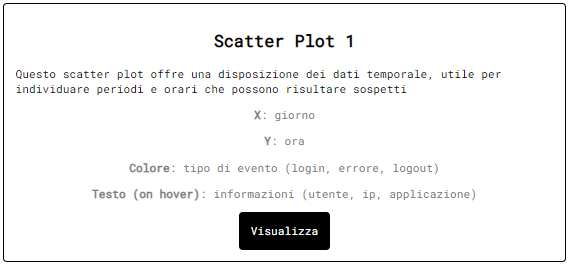
\includegraphics[width=1.0\textwidth]{scatterplot1.png}
	\caption{Informazioni Scatter Plot 1}
  \end{figure}
Questa prima tipologia di \textit{Scatter Plot} permette di individuare degli accessi sbagliati eseguiti in orari sospetti, quindi per esempio durante l'orario non di ufficio. Eseguendo un nuovo campionamento si può notare se queste anomalie persistono oppure se era un errore dovuto a quello specifico campionamento. In caso quella anomalia dovesse persistere si può posizionarsi sopra con il mouse e nelle informazioni vedere l'utente o gli utenti sospetti.
\begin{figure}[H]
	\centering
	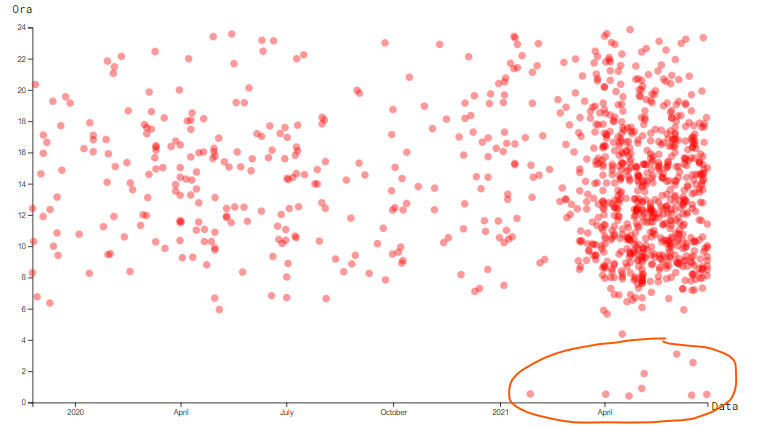
\includegraphics[width=1.0\textwidth]{scatter1anom.png}
	\caption{Accessi sospetti Scatter Plot 1}
  \end{figure}
\section{Scatter Plot 2}
\begin{figure}[H]
	\centering
	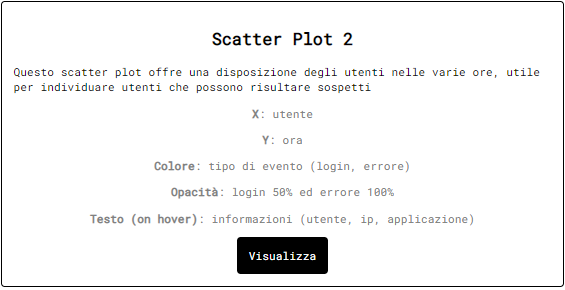
\includegraphics[width=1.0\textwidth]{scatterplot2.png}
	\caption{Informazioni Scatter Plot 2}
  \end{figure}
Questa seconda tipologia di \textit{Scatter Plot} permette di individuare un utente che ha una percentuale di accessi sbagliati più alta di quelli andati a buon fine, basta guardare le varie linee verticali che si riferiscono ad un singolo utente. Anche in questo grafico gli accessi sbagliati più sospetti sono quelli effettuati durante l'orario non di ufficio, indicato sull'asse y.
\begin{figure}[H]
	\centering
	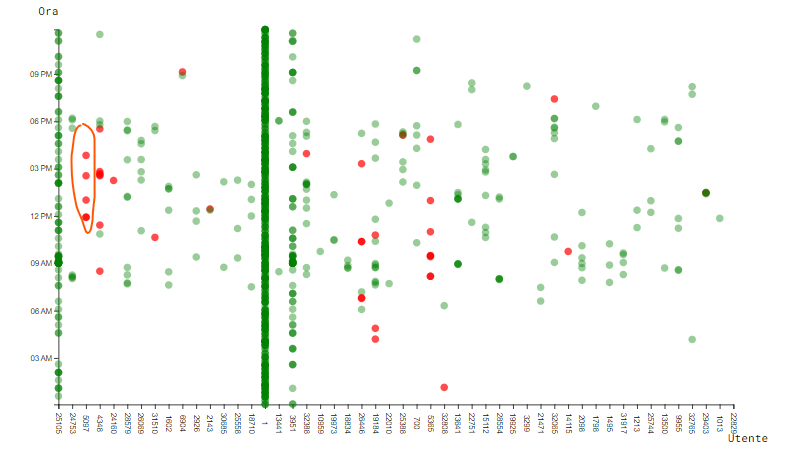
\includegraphics[width=1.0\textwidth]{scatter2anom.png}
	\caption{Utente sospetto Scatter Plot 2}
  \end{figure}
\section{Parallel Coordinates}
\begin{figure}[H]
	\centering
	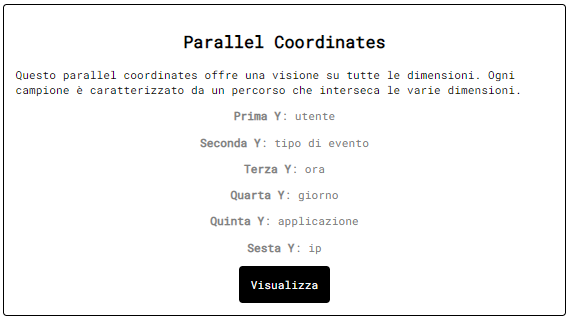
\includegraphics[width=1.0\textwidth]{parallelcoordinates.png}
	\caption{Informazioni Parallell Coordinates}
  \end{figure}
Questa tipologia di grafico offre una visione su tutte le dimensioni, infatti ogni asse verticale ne rappresenta una. È un grafico molto utile se si filtra per tipo di evento, in particolare login errato, perchè così facendo possiamo vedere il periodo in cui ne sono stati effettuati maggiormente e anche il tipo di applicazione dalla quale sono stati fatti.
\begin{figure}[H]
	\centering
	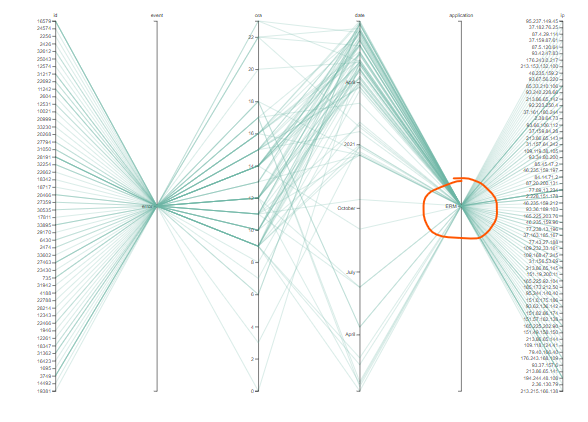
\includegraphics[width=1.0\textwidth]{parallelanom.png}
	\caption{Tipo di applicazione dalla quale vengono effettuati tanti errori di accesso}
  \end{figure}
\section{Sankey Diagram}
\begin{figure}[H]
	\centering
	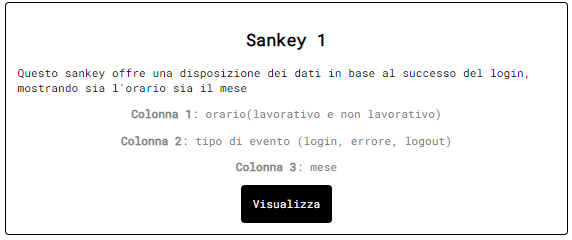
\includegraphics[width=1.0\textwidth]{sankeydiagram.png}
	\caption{Informazioni Sankey Diagram}
  \end{figure}
Questa tipologia di grafico è formata da barre dalle quali escono dei fasci. Si può notare nell'orario di ufficio e in quelo non di ufficio tramite la grandezza dei fasci uscenti la distribuzione di login, logout ed errori. È un grafico utile se si filtra per utente perchè permette di avere un quadro generale del suo comportamento e la distribuzione degli accessi.
\begin{figure}[H]
	\centering
	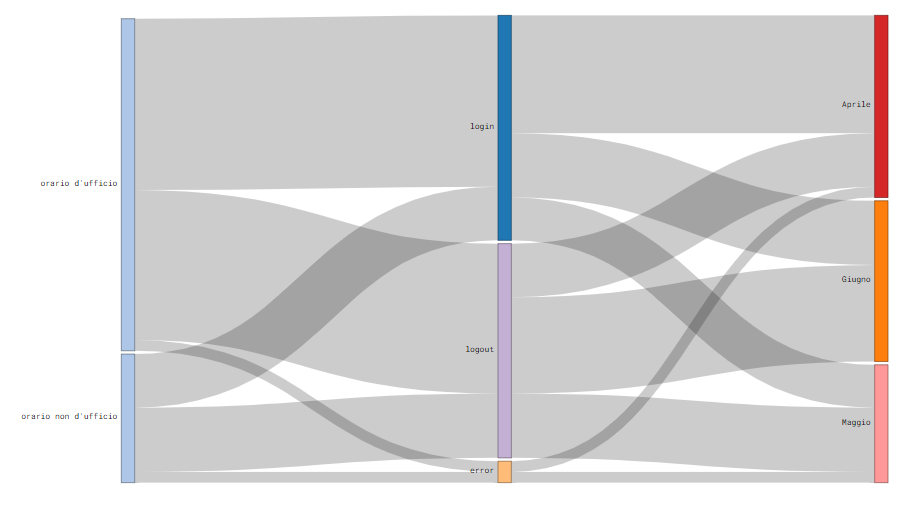
\includegraphics[width=1.0\textwidth]{sankeyutente21518.png}
	\caption{Accessi dell'utente 21518}
  \end{figure}
\section{Force Directed Graph}
